\subsection{Three or more addends 多个数字加法}
\begin{paracol}{2}
When there are thre or more addends, adding them one by one is the basic method. However there are also some tricks we can use to help solve
the problem more quickly. All of the tricks are based on Theorem \ref{thm:commutative}. We can add the easy addends first. 
\switchcolumn[1]
当计算三个或以上数的加法时,逐项相加是最基本的方法。但是对于一些有特殊特点的计算,有一些计算技巧可以来帮助我们。所有的技巧都是根据定理\ref{thm:commutative}。我们可以先计算简单的加和。
\end{paracol}
\begin{newthem}[Commutative property of addtion 加法交换律]
\label{thm:commutative}
changing the order of the addends does not change the result.\\
改变加法各项的顺序,计算结果不变。
\end{newthem}

\paragraph{Looking for a sum of 10  凑十法}
\ \  

\begin{paracol}{2}
We already know that the addition of the following $5$ pairs is $10$. We can use these results to do the computation quickly. 
\switchcolumn[1]
我们已经知道,下面的五组成对的数相加之和都等于$10$。利用这些结果可以使计算又快又准。
\end{paracol}
$$
\begin{aligned}
1+9=9+1=10,\quad & 2+8=8+2=10,\quad & 3+7=7+3=10\\
4+6=6+4=10,\quad & 5+5=10.
\end{aligned}
$$
\begin{example}
1+2+3+4+5+6+7+8+9+10
\end{example}
\begin{solution}
\begin{paracol}{2}
As the basic method, we can add them one by one.
\switchcolumn[1]
对于这道题,基础的方法是从左往右逐项相加。
\end{paracol}
$$
\begin{aligned}
1+2=3,\quad & 3+3=6,\quad & 6+4=10,\\
10+5=15,\quad & 15+6=21,\quad, & 21+7 = 28,\\
28+8=36,\quad & 36+9=45,\quad,& 45+10 = 55.
\end{aligned}
$$
\begin{paracol}{2}
The advantage of this method is that we can get all of the intermedia results. However it is complecated and easy to make mistakes. If one addition in one of the steps is wrong, it will be wrong after. And it is really difficult to find out where it goes wrong. The new method which looking for the sum of 10 could fix this problem.
\switchcolumn[1]
这种逐项相加的方法,好处是可以得到每一步的结果,但缺点是麻烦,容易出错;而且一步出错,以后步步都错。并且很难检查错误。若是利用凑十法,就可以克服这种缺点。
\end{paracol}

\begin{center}
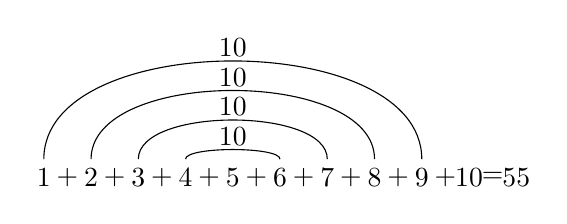
\begin{tikzpicture}[auto, node distance=0.3cm]
\node[] (1) {1};
\node[] (p1) [ right of=1] {$+$};
\node[] (2) [ right of=p1] {2};
\node[] (p2) [ right of=2] {$+$};
\node[] (3) [ right of=p2] {3};
\node[] (p3) [ right of=3] {$+$};
\node[] (4) [ right of=p3] {4};
\node[] (p4) [ right of=4] {$+$};
\node[] (5) [ right of=p4] {5};
\node[] (p5) [ right of=5] {$+$};
\node[] (6) [ right of=p5] {6};
\node[] (p6) [ right of=6] {$+$};
\node[] (7) [ right of=p6] {7};
\node[] (p7) [ right of=7] {$+$};
\node[] (8) [ right of=p7] {8};
\node[] (p8) [ right of=8] {$+$};
\node[] (9) [ right of=p8] {9};
\node[] (p9) [ right of=9] {$+$};
\node[] (10) [ right of=p9] {10};
\node[] (e) [ right of=10] {$=$};
\node[] (sum) [ right of=e] {55};
\draw (1)  .. controls +(up:1.9cm) and +(up:1.9cm) .. node [above=-2pt]{10} (9);
\draw (2)  .. controls +(up:1.4cm) and +(up:1.4cm) .. node[above=-2pt]{10} (8);
\draw (3)  .. controls +(up:0.9cm) and +(up:0.9cm) .. node[above=-2pt]{10} (7);
\draw (4)  .. controls +(up:0.4cm) and +(up:0.4cm) .. node[above=-2pt]{10} (6);
\end{tikzpicture}
\end{center}
\end{solution}

\paragraph{Looking for a sum of a whole number  凑整法}
\ \  

\begin{paracol}{2}
Some number pairs could add up to tens or hundreds. For example
\switchcolumn[1]
有些数相加之和是整十、整百的数,如:
\end{paracol}

\begin{align*}
1+19&=20, \quad & 11+19&=30,\\
12+28&=40, \quad & 12+38&=50,\\
23+37&=60, \quad & 33+37&=70,\\
34+46&=80, \quad & 44+46&=90,\\
15+85&=100, \quad & 45+55&=100.
\end{align*}

\begin{paracol}{2}
These results could help us in the computation.
\switchcolumn[1]
巧用这些结果,可以使那些较大的数相加又快又准。
\end{paracol}

\begin{example}
$1+3+5+7+9+11+13+15+17+19$
\end{example}
\begin{solution}
\begin{center}
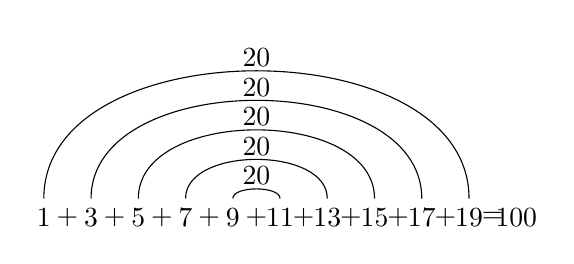
\begin{tikzpicture}[auto, node distance=0.3cm]
\node[] (1) {1};
\node[] (p1) [ right of=1] {$+$};
\node[] (3) [ right of=p1] {3};
\node[] (p2) [ right of=3] {$+$};
\node[] (5) [ right of=p2] {5};
\node[] (p3) [ right of=5] {$+$};
\node[] (7) [ right of=p3] {7};
\node[] (p4) [ right of=7] {$+$};
\node[] (9) [ right of=p4] {9};
\node[] (p5) [ right of=9] {$+$};
\node[] (11) [ right of=p5] {11};
\node[] (p6) [ right of=11] {$+$};
\node[] (13) [ right of=p6] {13};
\node[] (p7) [ right of=13] {$+$};
\node[] (15) [ right of=p7] {15};
\node[] (p8) [ right of=15] {$+$};
\node[] (17) [ right of=p8] {17};
\node[] (p9) [ right of=17] {$+$};
\node[] (19) [ right of=p9] {19};
\node[] (e) [ right of=19] {$=$};
\node[] (sum) [ right of=e] {100};
\draw (1)  .. controls +(up:2.4cm) and +(up:2.4cm) .. node [above=-2pt]{20} (19);
\draw (3)  .. controls +(up:1.9cm) and +(up:1.9cm) .. node[above=-2pt]{20} (17);
\draw (5)  .. controls +(up:1.4cm) and +(up:1.4cm) .. node[above=-2pt]{20} (15);
\draw (7)  .. controls +(up:0.9cm) and +(up:0.9cm) .. node[above=-2pt]{20} (13);
\draw (9)  .. controls +(up:0.4cm) and +(up:0.4cm) .. node[above=-2pt]{20} (11);
\end{tikzpicture}
\end{center}
\end{solution}

\begin{example}
$2+13+25+44+18+37+56+75$
\end{example}
\begin{solution}
\begin{center}

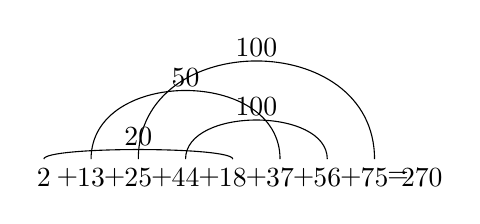
\begin{tikzpicture}[auto, node distance=0.3cm]
\node[] (2) {2};
\node[] (p1) [ right of=2] {$+$};
\node[] (13) [ right of=p1] {13};
\node[] (p2) [ right of=13] {$+$};
\node[] (25) [ right of=p2] {25};
\node[] (p3) [ right of=25] {$+$};
\node[] (44) [ right of=p3] {44};
\node[] (p4) [ right of=44] {$+$};
\node[] (18) [ right of=p4] {18};
\node[] (p5) [ right of=18] {$+$};
\node[] (37) [ right of=p5] {37};
\node[] (p6) [ right of=37] {$+$};
\node[] (56) [ right of=p6] {56};
\node[] (p7) [ right of=56] {$+$};
\node[] (75) [ right of=p7] {75};
\node[] (e) [ right of=75] {$=$};
\node[] (sum) [ right of=e] {270};
\draw (25)  .. controls +(up:1.9cm) and +(up:1.9cm) .. node [above=-2pt]{100} (75);
\draw (13)  .. controls +(up:1.4cm) and +(up:1.4cm) .. node[above=-2pt]{50} (37);
\draw (44)  .. controls +(up:0.9cm) and +(up:0.9cm) .. node[above=-2pt]{100} (56);
\draw (2)  .. controls +(up:0.4cm) and +(up:0.4cm) .. node[above=-2pt]{20} (18);
\end{tikzpicture}
\end{center}

\end{solution}
   \newpage